% Capítulo 1: as etapas que o navegador percorre para desenhar a página.
\documentclass[border=4pt]{standalone}
\usepackage[utf8]{inputenc}
\usepackage[T1]{fontenc}
% Estilo comum dos fluxogramas e diagramas de blocos.
\usepackage{tikz}
\usetikzlibrary{arrows.meta, positioning, calc, shapes.geometric, shapes.misc}
\definecolor{navy}{RGB}{23,45,80}
\definecolor{laranja}{RGB}{250,110,29}
\definecolor{cinzalogo}{RGB}{107,114,126}
\definecolor{azul}{RGB}{205,222,247}
\tikzset{
  base/.style={draw=navy, line width=0.9pt, font=\sffamily\small, align=center, inner sep=4pt},
  terminal/.style={base, rounded rectangle, fill=laranja!45, draw=laranja, minimum width=20mm, minimum height=7mm},
  processo/.style={base, rectangle, fill=laranja!12, minimum width=28mm, minimum height=8mm},
  decisao/.style={base, diamond, aspect=2.2, fill=azul, inner sep=1pt, minimum width=30mm},
  es/.style={base, trapezium, trapezium left angle=72, trapezium right angle=108,
             fill=white, minimum width=26mm, minimum height=8mm, trapezium stretches body},
  fluxo/.style={-{Stealth[length=2.2mm]}, navy, line width=0.9pt},
  rotulo/.style={font=\sffamily\small\bfseries, text=navy},
  legenda/.style={font=\sffamily\scriptsize, text=cinzalogo},
  resposta/.style={font=\sffamily\scriptsize\bfseries, text=navy},
}

\tikzset{
  arq/.style={base, rectangle, fill=white, font=\ttfamily\small, minimum width=18mm, minimum height=8mm},
  arv/.style={processo, minimum width=20mm},
  etapa/.style={processo, fill=azul, minimum width=19mm},
  nota/.style={legenda, align=center},
}
\begin{document}
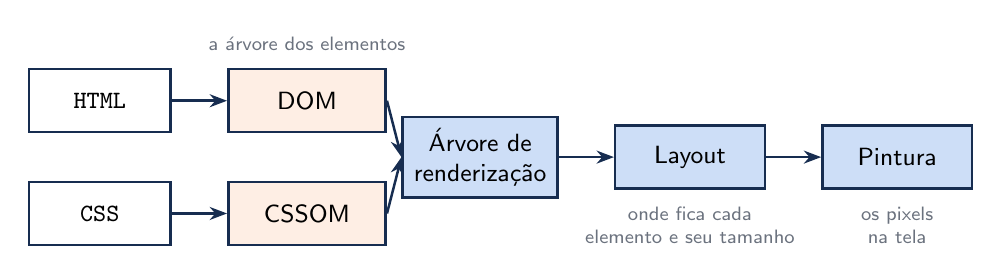
\begin{tikzpicture}[node distance=6mm and 7mm]
  \node[arq] (html) {HTML};
  \node[arq, below=of html] (css) {CSS};
  \node[arv, right=of html] (dom) {DOM};
  \node[arv, right=of css] (cssom) {CSSOM};
  \node[etapa, right=12mm of $(dom)!0.5!(cssom)$] (render) {Árvore de\\renderização};
  \node[etapa, right=of render] (layout) {Layout};
  \node[etapa, right=of layout] (pintura) {Pintura};

  \draw[fluxo] (html) -- (dom);
  \draw[fluxo] (css) -- (cssom);
  \draw[fluxo] (dom.east) -- (render.west);
  \draw[fluxo] (cssom.east) -- (render.west);
  \draw[fluxo] (render) -- (layout);
  \draw[fluxo] (layout) -- (pintura);

  \node[nota, below=1mm of layout] {onde fica cada\\elemento e seu tamanho};
  \node[nota, below=1mm of pintura] {os pixels\\na tela};
  \node[legenda, above=1mm of dom] {a árvore dos elementos};
\end{tikzpicture}
\end{document}
